% Rozdziały zaczynają się od "chapter"
\chapter{Introduction}
% Praca podzielona na mniejsze pliki włączane za pomocą input
% Zajrzyj do pliku tekst/wstep.tex
Liver cancer is a significant health concern, in 2020, it was the second most common cause of cancer-related death worldwide. Despite being one of the most common causes of death it is not the most common cancer, liver cancer accounted for $8.3\%$ of all deaths but only $4.7\%$ of all detected cases in 2020 \cite{sung_global_2021}. The reason for this increased mortality is the difficulty of diagnosing it at an early stage due to the lack of symptoms. Being a complex disease, the development and growth of liver cancer involve multiple microscopic and macroscopic changes in cell morphology, which are not yet fully understood. Chances of diagnosis at an early stage are provided by identification of these lesions on medical images of the liver. Some of the most common techniques for performing patient imaging include:
\begin{itemize}
    \item Ultrasound (US)
    \item Magnetic resonance imaging (MRI)
    \item Computed tomography (CT)
\end{itemize}

Each of these techniques has its own advantages and disadvantages related to aspects such as imaging cost, image quality and invasiveness to the patient \cite{li_application_2020}. The irregular shapes of the liver and tumor lesions make segmentation based on medical images a non-trivial task. Over the years, many techniques have emerged to ease this process. However, none of the classical methods allowed for the preservation of high accuracy of segmentation and for making it applicable to medical practices in high-volume settings. The need for high accuracy is obvious, while the possible scalability of the solution would allow for an increase in the detection of liver cancer among the entire population, and not only the wealthiest part would be able to pay for the time of specialized experts.


 In recent years, deep learning methods have revolutionized image processing techniques. Models developed based on these methods can automatically extract hierarchical representations of image features from raw input data. They can recognize complex patterns and representations found in images at different levels of abstraction \cite{anguera_impact_2018}. Given the level of complexity and the multidimensionality of medical images, methods based on deep learning are considered highly promising and likely to revolutionize medical radiology in the near future.

Accordingly, this work aims to summarize the current research and state of the art in detecting malignant lesions on medical images, focusing on methods using deep learning while mentioning classical ones. Apart from it the goal is to create a program that performs the automatic segmentation of CT images using deep learning and evaluate its performance.




% Można też wszystko pisać w jednym pliku ale będzie on duży
\chapter{State of the art and literature review}


% fragment nieużywany albo jeszcze niedodany można zakomentować
\section{Overview of Liver Tumor Segmentation Techniques} \label{overview_techniques}


We can divide traditional techniques for segmenting liver and tumor lesions into three categories:
\begin{itemize}
    \item Manual 
    \item Semi-automated
    \item Fully automated     
\end{itemize}

Manual segmentation involves contouring the pixels that border the liver or the tumor lesion. Originally done with a pencil, medical images are now saved as Digital Imaging and Communications in Medicine (DICOM) files, and radiologists doing the segmentation usually have access to tools that optimize the contouring. Despite this support, this approach further qualifies as manual. The most common tool for optimizing contouring is Snake model for Active Contouring \cite{kass_snakes_1988}. 

Semi-automated segmentation techniques require initialization by the user; the corresponding algorithm does the rest. Among the most popular methods are intensity-based approaches and the Graph-cut technique. The Seeded Region Growing (SGR)  \cite{fan_seeded_2005} algorithm can be mentioned for intensity-based techniques. The user initializes it by selecting a certain number of seed pixels in the object we want to segment, then based on intensity, neighboring pixels are added until the whole object is selected. Example of SGR can be seen on figure \ref{rys:sgr} .The graph-cut technique \cite{boykov_graph_2006} requires similar input from the user, in addition to which user must also select the grain of the area that is the background for the object of interest. The algorithm constructs a graph whose vertices are pixels and edges represent the relationships between them based on similarity and the structure of the whole image. The algorithm splits this graph to segment the area of interest.

\begin{figure}[!h]
	\centering \includegraphics[width=\linewidth]{rysunki/1-s2.0-S0030402619316031-gr5.jpg}
	\caption{Example of Seeded Region Growing. First row contains original CT images, second one points out which seed pixel were selected, last one results of segmentation. Image from  \textit{Liver segmentation based on region growing and level set active contour model with new signed pressure force function} by Lei Xu et al. }
	\label{rys:sgr}
\end{figure}

Automatic methods do not require any significant input from the user to perform segmentation. As an example, Statistical shape models (SSMs) \cite{heimann_statistical_2009}, based on predefined shapes of objects of interest, generate segmentation that does not deviate from them. Another example of such methods is techniques based on pixel classification. For this purpose, support vector machine models (SVMs) \cite{jie_lu_automatic_2012} or random forests models \cite{hadjiiski_3d_2015} are used. 




These aforementioned classical segmentation methods have significant limitations and drawbacks, described in detail in the context of performing liver volumetry in \cite{gotra_liver_2017}. As the main disadvantages of the manual approach, the article identifies intra-observer and inter-observer variability related to the subjectivity of segmentation. Another disadvantage mentioned in the article is the long time required to perform segmentation using this method (up to 90 minutes). The limited number of specialists in the field makes it unsuitable for large-scale applications. As for automatic and semi-automatic methods, the low robustness of these solutions, i.e., resistance to borderline cases such as the very unusual shape of the liver or deformations related to past surgeries, are indicated as disadvantages. In addition, the complexity of implementing these solutions is indicated. It should also be mentioned that the work of Akshat Gotra \cite{gotra_liver_2017} only dealt with liver segmentation and not liver tumor lesions. Tumors often have irregular shapes, unclear boundaries, and different levels of contrast compared to adjacent tissues, making manual segmentation a challenge that is prone to error even for experienced specialists. These factors also add to the disadvantages of the automatic and semi-automatic methods mentioned above.

Deep learning methods have revolutionized image segmentation by using neural networks to learn relevant features from an image automatically. Segmentation methods using deep learning can be divided into three categories:
\begin{itemize}
    \item Semantic segmentation --- is a type of segmentation in which each pixel is given a label with  a recognized class while individual instances of classes are not distinguished.
    \item Instance segmentation --- goes a step further than semantic segmentation by distinguishing between individual instances of classes. For example, each tree would be separately identified and segmented in a picture with several trees.
    \item Panoptic segmentation \cite{kirillov_panoptic_2019} --- is a relatively new type that combines semantic and instance approaches. Each pixel receives a semantic label indicating which class it belongs to and an instantaneous label indicating which instance it represents.
\end{itemize}
Semantic segmentation is usually used to detect liver cancer lesions.

Segmentation based on deep learning methods can be categorized as fully automated. This makes it possible to use solutions in clinical practice on a massive scale and allows access to diagnosis to a much wider group of people than could be the case with the use of manual or semi-automated methods. At the same time, deep learning methods have achieved much higher accuracy than traditional automatic methods \cite{liu_review_2021}. The performance of deep learning methods in segmentation can be compared to the manual work of expert radiologists \cite{hirsch_radiologist-level_2022}, which, for obvious reasons, requires more resources than an automatic solution. Despite the advantages above over traditional methods, applying deep learning methods in segmentation remains an active research area, and further improvements to this methodology appear with each passing year.



%%%%%%%%%%%%%%%%%%%%%%%%%%%%%%%%%%%%%%%%%%%%%%%%
\section{Deep Learning Architectures for Liver Tumor Segmentation}

Section describes the most critical types of deep learning model architectures designed for the semantic segmentation of medical images. In the following part, the reader can find a general description and achieved results in the segmentation of the liver and its cancerous lesions of such types of architectures as Convolutional neural networks (CNNs), U-Net and variations, Full convolutional networks (FCNs) and application of transfer learning.

\subsection{Convolutional Neural Networks}

Convolutional Neural Networks (CNNs) are a class of deep neural network models that are among the most widely used for image processing tasks. CNNs are used most often for classification and segmentation. Their essential element is convolutional layers performing convolution operations on an image and thus extracting its properties. They are usually followed by layers performing pooling operations, thanks to which we reduce the dimensions of the convolution output while preserving the most relevant information. Additional elements of the CNNs architecture are Rectilinear Unit (ReLU) activation and fully connected layers \cite{oshea_introduction_2015}. An example of CNN architecture for semantic segmentation of liver tumors can be seen on figure \ref{rys:cnn_arch}.

Wen Li in \cite{li_automatic_2015} described using CNNs in segmenting liver cancer lesions. The solution created was characterized by high accuracy and robustness. As a limitation of this approach, the authors mention segmenting tumors with inhomogeneous density and unclear boundaries.


\begin{figure}[!h]
	\centering \includegraphics[width=\linewidth]{rysunki/61314x7.png}
	\caption{Example of CNN architecture for liver tumor segmentation. Image from \textit{Automatic Segmentation of Liver Tumor in CT Images with Deep Convolutional Neural Networks} by Wen Li et ali.}
	\label{rys:cnn_arch}
\end{figure}

\subsection{U-Net and variants}

Ronneberg proposed the U-net architecture to segment biomedical images \cite{navab_u-net_2015}. The network consists of two parts: 
\begin{itemize}
    \item The left one is called the contracting path. 
    \item The right one is called the expensive path.
\end{itemize}
\label{ref:u-net}

The contracting path features a typical CNN architecture and acts as an encoder. It consists of repeated 3x3 convolution layers, each followed by a rectified linear unit (ReLU); after a block of two convolution layers, there is a 2x2 max-pooling layer with stride 2, which performs downsampling. After each downsampling, the number of feature maps is doubled. This causes U-Net to learn fewer features at higher resolution and more at lower resolution. 

The expensive path consists of blocks that first increase the resolution of the feature map through upsampling, followed by a 2x2 convolution (referred to as "up-convolution") that reduces the number of feature channels by half. This is then followed by merging with the appropriately trimmed feature map from the contracting pathway and, finally, two consecutive 3x3 convolutions, each succeeded by a Rectified Linear Unit (ReLU) activation function.

The critical element distinguishing U-Net from typical auto-encoders is the connections between corresponding levels in the contracting and expensive paths. These are called skip connections and function for every but the last level. Their role is to convey information about what the network saw when processing the image, that is, what feature maps it extracted, at a given level of the contracting path to the corresponding level of the expensive path. The U-net architecture is presented in \\ figure \ref{rys:u_net_arch}.

\begin{figure}[!h]
	\centering \includegraphics[width=\linewidth]{rysunki/u-net-architecture.png}
	\caption{U-Net architecture for image segmentation. Image from \textit{U-Net: Convolutional Networks for Biomedical Image Segmentation} by Olaf Ronneberger et ali} 
	\label{rys:u_net_arch}
\end{figure}

The original U-Net architecture is usually modified for the liver cancer segmentation task by using other skip connections and adding new pathways. Taking the Dice coefficient in coping with liver cancer segmentation with CT images from the LiTS public dataset \cite{bilic_liver_2023} as a quality metric, the best existing variant is the mU-Net \cite{seo_modified_2020}, it has detected more than $90\%$ of cancer lesions present in dataset.

\subsection{Fully Convolutional Networks}

The Fully Convolutional Network (FCN) architecture presented by Long \cite{long_fully_nodate} is used for the task of semantic segmentation. The element that distinguishes FCNs from CNNs is the lack of a fully connected layer. Instead, FCNs uses upsampling via convolution operations and returns as the end result in the probability of each pixel of the input image belonging to the given classes. An example of architecture can be seen in the figure \ref{rys:fcn_arch}. Despite being created as a tool for semantic segmentation in general, researchers very often use FCN to segment medical images, including liver cancer lesions (\cite{christ_automatic_2017}, \cite{carneiro_fully_2016}), and it achieves good results in this task.

\begin{figure}[!h]
	\centering \includegraphics[width=\linewidth]{rysunki/new_alex-model.jpg}
	\caption{Fully Convolutional Networks architecture. Image from \textit{Fully Convolutional Networks for Semantic Segmentation} by Jonathan Long et ali. } 
	\label{rys:fcn_arch}
\end{figure}

\subsection{Transfer Learning}

All the described deep learning methods require a dataset on which they can learn. In the context of segmenting liver tumor lesions from CT images, this means a set of such images with corresponding liver and tumor lesions segmentations. The preparation of such a dataset is time-consuming and costly because it requires the involvement of specialists in this domain; it was described earlier in the context of traditional segmentation methods. Transfer Learning is a technique that can improve the accuracy of deep learning models lacking sufficient learning data \cite{zoetmulder_domain-_2022}. Additional advantages of this technique can be the reduction of model training time, which in some cases can take up to weeks \cite{gut_benchmarking_2022}. The technique involves transferring knowledge from an already trained model to the one we want to train. For the transfer to be effective, both models should be related to the same domain and task \cite{gut_benchmarking_2022}, i.e., segmentation of CT images. As mentioned by Riaan Zoetmulder in \cite{zoetmulder_domain-_2022}, in the context of medical image segmentation, the most common example of Transfer Learning is the use of an already trained encoder. The authors report that for this purpose, the most commonly used for this purpose are 
constant and repetitive structures (VGG variants), inception modules (GoogleNet, Inception V2, Inception V3), residual modules (ResNet variants) and dense blocks (DenseNet variants).

\section{Datasets and Evaluation Metrics}

\subsection{Commonly used datasets for liver tumor segmentation} \label{datasets}

Collecting enough data is necessary to create a segmentation model based on deep learning. The quality of the segmentation performed depends on the quality of the medical images and the labels developed by experts indicating which pixels the liver and its cancerous lesions are located \cite{liu_review_2021}. Popular publicly available datasets are :
\begin{itemize}
    \item MICCAI 2017 Liver Tumor Segmentation (LiTS) Challenge Dataset \cite{bilic_liver_2023}: This dataset encompasses contrast-enhanced CT images annotated manually for tumors. It comprises 130 abdominal CT scans featuring a total of 201 liver lesions. \label{sec:lits}
    \item CHAOS (Combined Healthy Abdominal Organ Segmentation) Dataset \cite{kavur_chaos_2021}: While primarily designed for organ segmentation, this dataset also includes annotations for liver tumors. It offers CT and MRI scans with annotations for various abdominal organs and tumors, including those of the liver.
    \item PAIP 2019 Challenge Dataset \cite{kim_paip_2021}: One of the few datasets with whole-slide images. It consists of one hundred cases, and each has a liver tumor.
    \item 3Dircadb: This dataset presents 3D abdominal CT scans featuring diverse liver lesions. It has been extensively utilized for liver tumor segmentation endeavors.
\end{itemize}


\subsection{Evaluation metrics for assessing segmentation performance}

To evaluate a given segmentation and to be able to compare it with another, it is necessary to establish some objective metric. In medical image segmentation, a manually performed segmentation of liver and tumor lesions by a qualified radiologist is considered Ground Truth. Popular metrics that we can include are:

\begin{itemize}
    \item \textbf{Dice Similarity Coefficient (DSC)} \begin{equation}
    DSC = \frac{2 \times |Prediction \cap Ground\,Truth|}{|Prediction| + |Ground\,Truth|} 
\end{equation}

    \item \textbf{Jaccard Index (IoU)}
    \begin{equation}
     IoU = \frac{|Prediction \cap Ground\,Truth|}{|Prediction \cup Ground\,Truth|} \end{equation}

     \item \textbf{Sensitivity} or \textbf{ True Positive Ratio (TPR)}
    \begin{equation}
     TPR = \frac{TP}{TP + FN}
 \end{equation}

     \item \textbf{Precision} 
    \begin{equation}
      PPV = \frac{TP}{TP + FP} 
 \end{equation}


 \item \textbf{Specificity} or \textbf{ True Negative Ratio (TNR)}
    \begin{equation}
      TNR = \frac{TN}{TN + FP}
 \end{equation}


 \item \textbf{Accuracy} 
    \begin{equation}
      Accuracy = \frac{TP + TN}{TP + TN + FP + FN} 
 \end{equation}
\end{itemize}

Explanation of the symbols used in the above formulas:
\begin{itemize}
    \item \textbf{Prediction} - A set of pixels classified as a segmented object by the model.
    \item \textbf{Ground Truth} - A set of pixels classified as a segmented object by qualified radiologist.
    \item \textbf{TP} - Number of true positive pixels.
    \item \textbf{TN} - Number of true negative pixels.
    \item \textbf{FP} - Number of false positive pixels.
    \item \textbf{FN} - Number of false negative pixels.
    
\end{itemize}

Popular metrics for evaluating medical segmentation can be divided into those based on the intersection of sets and those based on the confusion matrix.




\subsection{Challenges in dataset selection and evaluation}

Among the biggest challenges in selecting a dataset are the diversity of the data and the quality of the annotations. A wide range of shapes of the liver itself should be represented, as well as tumor lesions. There are also different types of tumors, primary and secondary, which should be included in our collection. The variety of data on which the model will learn leads to a highly generalizable model. The difficulty in providing it is, among other things, related to patient privacy issues. The challenge of annotation quality is related to the disadvantages of manual segmentation already mentioned in earlier sections.


High diversity characterizes the LiTS dataset:  "cohort covers diverse types of liver tumor diseases, including primary tumor disease (such as hepatocellular carcinoma and cholangiocarcinoma) and secondary liver tumors (such as metastases from colorectal, breast and lung primary cancers). The tumors had varying lesion-to-background ratios (hyper- or hypo-dense). The images represented a mixture of pre- and post-therapy abdominal CT scans and were acquired with different CT scanners and acquisition protocols, including imaging artifacts (e.g., metal artifacts) commonly found in real-world clinical data." \cite{bilic_liver_2023}. 

Data augmentation techniques are also a solution that will allow us to get diversity. They involve artificially creating variations of the existing data (e.g., rotations, flips).

As for the challenges of evaluative metrics, the most significant is that none perfectly captures clinical practice's relevance. For instance, a small segmentation error might be clinically insignificant but heavily penalized by some metrics.

\section{Preprocessing techniques}

For models based on deep learning methods to achieve high segmentation accuracy, medical images created using CT and MRI usually undergo preprocessing \cite{islam_evaluation_2021}. This is done to, among other things, remove unnecessary artifacts associated with, for example, the devices that performed the imaging. Additional goals are to increase the visibility of elements of interest and thus reduce those not of interest. This section describes the most essential techniques used to perform image preprocessing.


\subsection{Hounsfield Unit Windowing}
Hounsfield units (HU) were named after Dr. Hounsfield, the creator of computed tomography. They are intended to represent the density of a given tissue; water has been given a value of 0, denser tissues have a positive value (e.g., blood, liver, and brain), and sparser tissues (e.g., air and fat). Dicom file images used to represent the result of a CT scan have pixels with a value in range $[-1014, 4000]$. To make it possible for the human eye to see the details associated with the area of interest, their values are limited to a specific interval using an operation called HU windowing. The operation has two parameters: Window level (WL), which determines the average HU value of the tissues whose visibility we want to improve, and Window width (WW), which determines the size of the range of HU values \cite{whalen_slice_2003}. As Muhammad Islam points out in \cite{islam_evaluation_2021}, the ranges of HU values observed in the various studies are $[-100, 400]$, $[75, 175]$, and $[-200, 250]$. The parameters of HU windowing are the hyperparameter of the model performing segmentation and should, therefore, be selected during hyperparameter tuning. An example of the HU windowing effect can be seen in figure \ref{rys:hu windowing}.

\begin{figure}[!h]
	\centering \includegraphics[width=\linewidth]{rysunki/Abdominal-CT-window-settings-basic.png}
	\caption{Examples of CT image with different windowing parameters. As we can see on each variant we are able to see different anatomical elements. The image comes from web article \href{https://litfl.com/abdominal-ct-windows-basics/}{Abdominal CT: Windows basics}.  } 
	\label{rys:hu windowing}
\end{figure}


\subsection{Histogram equalization}
An image's histogram is a graphical representation of the intensity distribution of the pixels that make up the image. It is assumed that images whose pixels cover the entire range of possible intensities are characterized by good contrast and thus make it easier to see the details of the related information not contained in the image. Histogram equalization operations are used to improve an image whose pixels do not cover the entire range of possible values. This operation "stretches" the image's histogram to cover all possible values. There are various methods of implementing this operation while Priyanka Garg in \cite{garg_comparative_2017} points to Cumulative Histogram Equalization as the best. A variation of histogram equalization is adaptive histogram equalization. In the adaptive method, several histograms are calculated for different sections of the original image. As Igor Rafael S. Valente pointed out in \cite{valente_automatic_2016}, this method is most often used in medical image segmentation. An example of the effect of adaptive histogram equalization can be seen in figure \ref{rys:hist_eq}.



\begin{figure}[!h]
	\centering \includegraphics[width=\linewidth]{rysunki/Example-of-an-adaptive-histogram-equalization-of-an-image-from-LIDC-IDRI-database-a-is.png}
	\caption{Example of an adaptive histogram-equalization of an CT scan from LIDC-IDRI database: (a) is the original image and (b) is the image after adaptive histogram equalization. Graphic from  \textit{Automatic 3D pulmonary nodule detection in CT images: A survey} by Igor Rafael S. Valente et ali.}
	\label{rys:hist_eq}
\end{figure}
\subsection{Data normalization}

Normalization aims to bring values from the entire data set to a standard scale while preserving their differences. This is particularly important when working with neural networks. Normalization makes the algorithms used in training them converge faster. In addition, bringing all features to the same scale means that every feature  has the same effect on model performance. Without this step, higher-scale features could dominate the network learning process. When working with CT images, there is also the possibility that they come from different devices performing the scans. The brightness scale of scans on different devices may differ; therefore, bringing them to the same scale is necessary \cite{truong_medical_2018}. There are various normalization techniques, such as min-max normalization, z-score normalization, decimal normalization, and logarithmic normalization. Z-score normalization is often used to segment liver cancer tissues \cite{islam_evaluation_2021}.


\subsection{Image denoising}

Denoising CT images is a complex issue to which many studies have been devoted, and many techniques have been developed. An example of an in-depth study regarding this issue is the work of Manoj Diwakar and Manoj Kumar \cite{diwakar_review_2018}. As the authors point out, due to the statistical uncertainty in each of the physical measurements made in computed tomography, the occurrence of noise in CT images is inevitable. It is necessary to use denoising methods. However, there is a tradeoff between noise reduction and preservation of medically relevant diagnostic information in the images. There are various methods for this purpose, each with certain disadvantages and limitations, so several are often used. Denoising methods can be divided into two categories: those based on the spatial domain and those based on the transform domain. For example, we can mention linear filters such as mean and median as examples of spatial methods. As for transform methods, wavelet-based denoising \cite{chen_wavelet-based_2013} is an example of such a technique. In the figure \ref{rys:denoise}, we can see an example of the result of denoisng.

\begin{figure}[!h]
	\centering \includegraphics[width=\linewidth]{rysunki/CT-scan-of-the-upper-abdomen-original-and-result-of-denoising.png}
	\caption{Example of the result of denoising a scan showing the abdominal , on the left is the original image and on the right is the result of denoising. Graphic from \textit{Pointwise adaptive estimation for robust and quantile regression} by Markus Reiß et ali.}
	\label{rys:denoise}
\end{figure}


\section{State-of-the-Art Studies and Results}
As mentioned in the introduction, manual segmentation of liver tumor lesions is a complex and time-consuming task. The combination of difficulty and time-consumingness further increases the risk of human error. In recent years, many automated solutions have appeared in machine learning, while highly accurate segmentation of tumor lesions has not been achieved by any of them. Currently, the most promising methods based on deep learning regarding scalability and segmentation accuracy are the most promising ones. The section \ref{recent_studies} describes recent research presenting the current state of knowledge related to the use of deep learning for liver cancer detection. The section \ref{seg_competitions} describes international competitions related to segmentation of the liver and its malignant lesions.




\subsection{Recent studies about deep learning methodologies for liver tumor segmentation}
\label{recent_studies}
Hameedur Rahman et al. in \cite{rahman_deep_2022} examined the effectiveness of the ResUNet network in segmenting the liver and its tumor lesions. ResUNet is an architecture in which the Res-net architecture replaces the left part of the U-Net. The authors tested this network on a public set of 3D-IRCADb-1 CT scans, achieving highly accurate segmentation with a Dice coefficient of $99.2\%$. Segmentation errors were associated with false positive predictions, which is better than false negatives from a clinical application point of view. In addition, the proposed solution works quickly, which allows it to be applied on a massive scale.
\label{ref:state_of_art}
Lingyun Li and Hongbing Ma proposed a similar architecture in \cite{li_rdctrans_2022}. The authors improved the original U-net architecture only on the left side. The original encoder was replaced by a hybrid composed of three modules: ResNeXt50 and dilated convolution transformers to improve performance. The resulting architecture was named RDCTrans U-Net. It was tested on a set of LiTS and achieved a Dice coefficient of $89.87\%$ in liver cancer segmentation.


Hyunseok Seo in \cite{seo_modified_2020} pointed out the following drawbacks of the classic U-Net architecture:
\begin{itemize}

    \item Extracted features are often blurred because of the possibility of transferring duplicate feature maps via skip connections.
    \item The high-level features extracted from the network do not contain enough high-resolution edge information, which leads to wrong predictions.
    \item Optimizing pooling operations to extract high-level global features is difficult because their number depends on the size of the image.
\end{itemize}
To solve these problems, the authors proposed adding a residual path with deconvolution and activation functions to skip connections. The network modified in this way was named mU-Net. Its performance in the context of liver tumor segmentation was tested on the LiTS and 3Dircadb datasets; it achieved $89.72\%$ and $68.14\%$ Dice coefficients, respectively.

Devidas T. Kushnure and Sanjay N. Talbar in \cite{kushnure_ms-unet_2021} proposed modifications to the U-Net architecture by adding a multiscale feature extractor. As a result, the network's reception capabilities have been improved; it can perform global and local feature extraction more granularly. The architecture thus created was named MS-UNet and tested on the 3Dircadb collection; it achieved a Dice factor of $84.15\%$ in the liver cancer segmentation task. In addition, the architecture has a lower computational complexity than the original one.

Sultan Almotairi and others in \cite{almotairi_liver_2020} presented an alternative approach to modifications to the U-net architecture. They used a modified SegNet, an architecture consisting of an encoder and decoder for semantic segmentation, to detect liver cancer. The model proposed by the authors detects most tumor tissues with an accuracy above $86\%$ for tumor classification on the 3D-IRCADb-01 dataset.

Most solutions that achieve good results in segmenting liver cancer lesions are based on 2d images. Three-dimensional CT scans are not used as input for two main reasons:
\begin{itemize}
    \item It significantly limits the amount of data available.
    \item Training the network on such data would require significant computational resources.
\end{itemize}
However, there are examples of networks based on 3D scans that achieve good results. 

Jianpeng Zhang et al. at \cite{zhang_light-weight_2019} presented a Light-Weight Hybrid Convolutional Network, which solved the previously mentioned problems of 3d image processing networks. The computational complexity is reduced by using two-dimensional convolution, which reduces the complexity, and then using three-dimensional convolution. An additional optimization they proposed is depthwise and spatiotemporal separate factorization for 3D convolutions. Their solution was evaluated on the LiTS and 3D-IRCADb dataset and achieved a Dice per case coefficient of $73\%$ and $94.1\%$, respectively, in the cancer lesion segmentation task.

Another good example of a solution based on three-dimensional input is described by Lu Meng et al. in \cite{meng_liver_2020}. They proposed a three-dimensional dual-path multiscale convolutional neural network. The use of a dual path balances the requirement of computational resources and segmentation accuracy. They tested their solution on the LiTS dataset and achieved a Dice coefficient of $68.9\%$ in the cancer lesion segmentation task.

\subsection{Segmentation competitions}
\label{seg_competitions}
Starting in 2007 and SLiver07, international competitions called segmentation challenges are held worldwide. These challenges are organized by multidisciplinary organizations and are designed to test different liver tumor segmentation techniques on the same dataset. However, classical methods were initially used for these challenges, such as the SSM models mentioned in the section \ref{overview_techniques}; as of 2016, mainly deep learning-based methods are used. This section will summarize the results of the most critical challenges; the datasets created for them are described in \ref{datasets}.
These challenges are very important from the point of view of evaluating the state of the art on this issue because they standardize solution evaluations by using one metric, the same dataset and running them on one computing environment.

\subsubsection{LiTS benchmark challenge 2017}
The LITS challenge \cite{bilic_liver_2023} was organized in collaboration between ISBI 2017 (IEEE International Symposium
on Biomedical Imaging) and MICCAI 2017 (Medical Image Computing
and Computer-Assisted Intervention). The goal of ISBI was to segment liver tumor tissues; additional goals set by MICCAI were to segment the liver itself and estimate tumor burden. Most of the solutions proposed by the challenge participants were based on deep learning. Evaluation of the segmentations was performed using the Dice coefficient. Summarizing all the results, the participants' solutions performed better in liver segmentation and achieved the best dice score of about $0.96$. Cancer lesion segmentation performed worse; J. Zou proposed the solution that achieved the best Dice score ($0.7$) and was a neural network based on Cascaded U-Nets architecture.
\subsubsection{CHAOS challenge 2019}

Combined Healthy Abdominal Organ Segmentation (CHAOS) \cite{kavur_chaos_2021} challenge was organized as part of the ISBI mentioned above, but the 2019 edition. The challenge featured five categories related to the segmentation of the liver and other abdominal organs from CT and MRI images. This selection of tasks was to get participants to create a universal solution capable of segmenting different organs based on images of different types. From the point of view of clinical practice, solutions with high generalization are very beneficial. An essential overall conclusion from the challenge is that solutions for a single modality (CT/MRI) are doing much better than those for multiple modalities. Additionally, most solutions performed much worse for segmenting multiple organs than just the liver, although there were exceptions to this trend. Despite not addressing the issue of segmentation of tumor lesions in the challenge, thanks to the conclusions above and the number of submissions (more than 550), the event significantly impacted the current state of knowledge and research directions.


\subsubsection{PAIP challenge 2019}
Pathology Artificial Intelligence Platform (PAIP) \cite{kim_paip_2021} was organized as part of MICCAI 2019. A dataset of whole-slide images (WSIs) was made available to participants. The organizers aimed to fill research gaps in the digital pathology field. Participants were faced with two tasks: segmenting liver tumor tissues and estimating real tumor burden. All submitted solutions were based on deep learning methods and were mainly variants of the U-Net architecture. The Jaccard index was used to evaluate the solutions in the segmentation task; the best score was 0.78.





%\input{tekst/donapisania}

\chapter{Practical example of DL based CT images segmentation}

This chapter describes the application I developed to segment tumor lesions using deep learning methods. The following sections describe the methodology of the solution, the implementation details, the parameters used, and the evaluation of the solution in the segmentation task.



\section{Dataset and preprocessing description}


The LiTS dataset was used to develop the solution and evaluate it. This dataset is described in section \ref{sec:lits}. The three-dimensional scans were randomly divided into training and testing data in proportions of 70/30, respectively, translating into 91 scans for training and 40 for testing.

In order to increase the amount of data, the three-dimensional scans were used to produce two-dimensional images called scan slices. Only every second slice was used, which still generated 21198 and 8158 training and testing images, respectively. The resulting images were single-channel grayscale. They were converted to three-channel images in RGB format to include more information in the images while emphasizing those of the liver. The individual channels were obtained as follows:
\begin{enumerate}
    \item The original grayscale image was subjected to HU windowing with a window level equal to 60 and window width equal to 200.
    \item The original grayscale image was subjected to histogram equalization.
    \item The original grayscale image was subjected to HU windowing with a window level equal to 30 and window width equal to 150.

\end{enumerate}

The values used as windowing parameters were chosen to increase the segmentation accuracy as much as possible. Since evaluating the solution for a given parameter value is very time-consuming, the issue has not been exhausted, and further research could be undertaken. The effect of the described processing can be seen in the figure \ref{fig:preproc_effect}.

\begin{figure}%
    \centering
    \subfloat[\centering Scan slice in greyscale]{{\includegraphics[width=5cm]{rysunki/orignal.jpg} }}%
    \qquad
    \subfloat[\centering Scan slice in RGB scale]{{\includegraphics[width=5cm]{rysunki/volume-0_slice_0.jpg} }}%
    \caption{Comparison of scan slice before and after preprocessing}%
    \label{fig:preproc_effect}%
\end{figure}


The model described in the following section also normalize and resize to 128x128 each input image.
\section{Methodology}
\subsection{Model architecture}

The U-Net architecture with ResNet34 as the backbone was used as the model for segmentation. Three components can be distinguished, occurring in sequence, of which the network is composed:
\begin{enumerate}
    \item ResNet34 that acts as an encoder.
    \item Bottleneck consisting of a layer of BatchNorm, ReLu, and a layer of double convolution.
    \item Decoder consisting of blocks from the classic U-Net architecture.
\end{enumerate}

Corresponding blocks from components 1 and 3 are connected via skip connections according to the assumptions behind the u-net architecture described in the section \ref{ref:u-net}. In the case of Resnet34, transfer learning was applied, a model with pre-trained weights was used. The model takes as input a batch of 16 images of size 128x128 and returns the probability that each pixel belongs to one of three classes:
\begin{enumerate}
    \item Background
    \item Liver
    \item Liver Tumor
\end{enumerate}
The class with the highest probability is the one to which the pixel belongs according to the model. Figure \ref{rys:my_arch} is the architecture of the model used; this visualization was made for a different task of segmentation of the compound, so the dimensions of the input of each layer are different.
\begin{figure}[!h]
	\centering 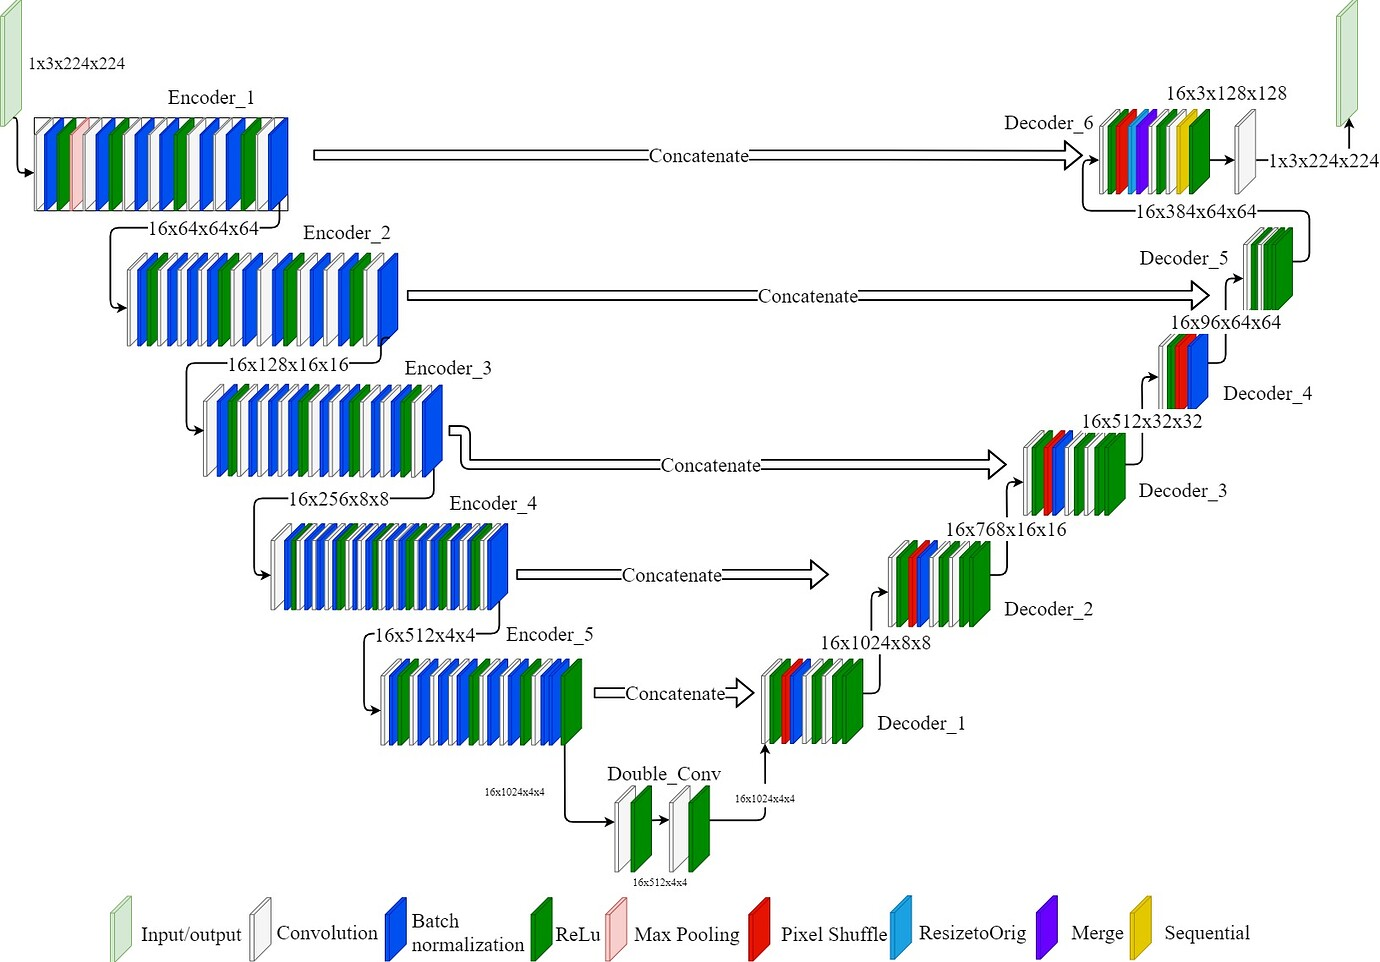
\includegraphics[width=\linewidth]{rysunki/135d5facd772ae16cee7360d0a0bbea8c74d5398_2_1380x962.jpeg}
	\caption{Architecture of network used in segmentation task. The image was created by user Adleman as part of discussion about this architecture on fastai framework forum \href{https://forums.fast.ai/t/u-net-with-resnet34-backbone/85744/4}{U-Net with ResNet34 backbone}.}
	\label{rys:my_arch}
\end{figure}

\subsection{Training Process}
As mentioned, the training has been conducted on a random subset representing $70\%$ of the total data. In addition, the data came to the model in batches of 16 images in size. An example of such a series can be seen in figure \ref{rys:batch}.

\begin{figure}[!h]
	\centering \includegraphics[width=\linewidth]{rysunki/another_batch.png}
	\caption{Example batch of training data. Segmentation masks have been overlaid on the input images, with red marking the liver and pink marking the tumor tissues.}
	\label{rys:batch}
\end{figure}
The hyperparameters used when training the network are listed in table \ref{tab:Hyperparameters}. For a larger number of epochs, the model did not significantly improve the operation, which is why this value was chosen. In the case of the loss function - its choice is arbitrary. However, exploring similar solutions on the Internet is one of the most common choices. In the case of learning rate, its value was chosen based on the LR range test described by Leslie Smith in \cite{smith_cyclical_2017}. This method selects the optimal learning rate based on going through one epoch of the model, changing the value of the learning rate during, and noting the corresponding value of the loss function. A randomly selected $20\%$ of the training data validates the model during training. For each epoch, the Dice coefficient achieved by the model in segmentation is also calculated.


 
\begin{table}[h!]
    \centering
    \begin{tabular}{|c|c|c|c|c|}
    \hline
        Hyperparameter & value  \\
        \hline 
        Number of epochs & 5 \\
        \hline
        Learning rate & 0.000091\\
        \hline
        Loss function & Cross-entropy\\
        \hline
    \end{tabular}
    \caption{Hyperparameters used for training networks }
    \label{tab:Hyperparameters}
\end{table}




\subsection{Testing}
A segmentation task was performed on a test data set to test the developed model. Based on the results, three evaluation metrics were used to examine how the model performed in variously defined tasks. The following metrics were used:
\begin{itemize}
    \item Dice coefficient
    \item Accuracy
    \item Precision
\end{itemize}
\label{model_testing}
These metrics were calculated for three different problems that the model is capable of solving:
\begin{enumerate}
    \item Segmentation of liver cancer lesions pixel-wise.
    \item Classification of whether a given input image shows a liver with cancer lesions.
    \item Classification of whether a patient has liver cancer lesions.
\end{enumerate}
The motivation for evaluating the model's performance in the context of problem number one is obvious. However, from the point of view of the practical applicability of such solutions, problems two and three are also significant. As mentioned in the introduction of this work, the reason for the high mortality rate of liver cancer is the problematic diagnosis of patients at an early stage of the disease. Gaining information about the existence of liver cancer tissues is, therefore, very valuable even if these lesions' segmentation is of low quality.
\section{Results}

\subsection{Training}

It took 4 hours and 36 minutes to train the model. The calculations took place on the CPU. The exact hardware specifications are described in the following section. The figure \ref{rys:plot_loss} shows the changing value of loss during training, both for the training and validation sets. In the figure \ref{rys:dice_training}, you can see the changing value of the Dice coefficient; this is a coefficient calculated for multi-class segmentation so that the segmentation efficiency of the liver itself is also included in this result. In figure \ref{rys:example_segs}, we can see the segmentation results performed on a specific random sample of data from the training data.



\begin{figure}[!h]
	\centering \includegraphics[width=0.7\linewidth]{rysunki/training_loss.png}
	\caption{Plot visualizing how values of training and validation loss changed during model training.}
	\label{rys:plot_loss}
\end{figure}

\begin{figure}[H]
	\centering \includegraphics[width=0.7\linewidth]{rysunki/dice_multi_class_training.png}
	\caption{Plot visualizing how value of Dice coefficient for multi-class segmentation changed during model training.}
	\label{rys:dice_training}
\end{figure}

\begin{figure}[H]
	\centering 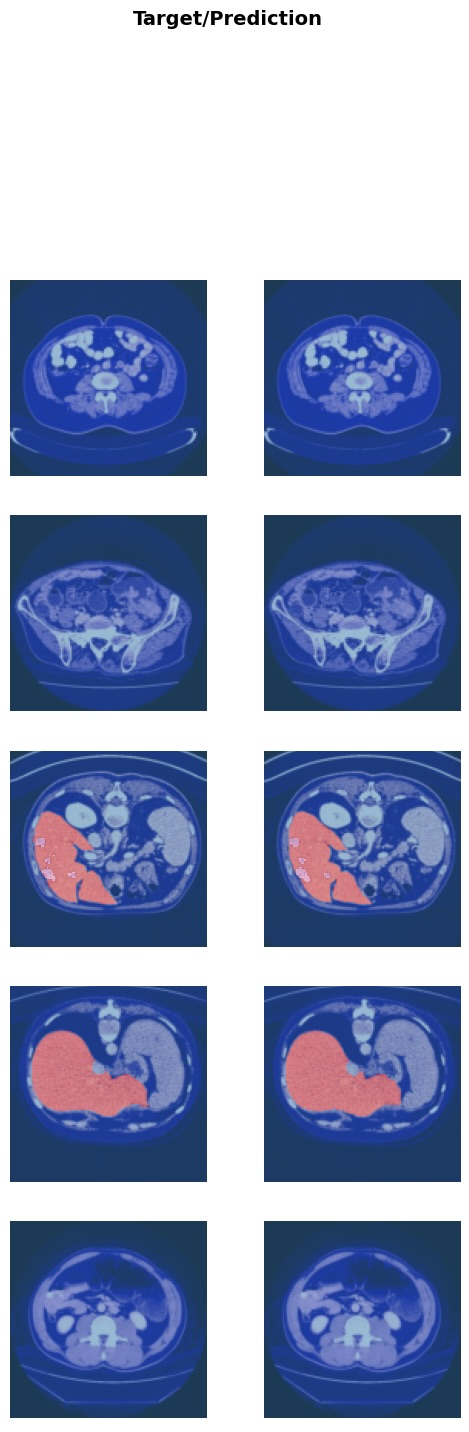
\includegraphics[scale=0.5]{rysunki/predykcje_modelu.jpeg}
	\caption{Segmentation performed on training set during model training. Red color marks the liver and pink tumor lesions}
	\label{rys:example_segs}
\end{figure}

\subsection{Testing}

It took about 0.5 seconds for the model to perform segmentation for one batch of test data. As described in the \ref{model_testing}, the same set of metrics was calculated for three different problems. The \ref{tab:metrics_prob_1} table presents the results that the model obtained in segmenting liver cancer lesions; these values refer to correctly classified pixels. In the \ref{tab:metrics_prob_2} table are presented the results that the model obtained in classifying a single input image as one with cancerous lesions. The \ref{tab:metrics_prob_3} table presents the results in classifying a patient with cancerous lesions. Figure \ref{fig:no_detected} shows an example of segmentation that did not detect existing tumor lesions. Instead, the figure \ref{fig:detected} shows a segmentation that detected existing lesions. Analysis of the results obtained is included in the next section.



\begin{table}[h!]
    \centering
    \begin{tabular}{|c|c|c|c|c|}
    \hline
        Metric & value  \\
        \hline 
        Accuracy & $0.99$ \\
        \hline
        Precision & $0.92$\\
        \hline
        Dice coefficient & $0.85$\\
        \hline
    \end{tabular}
    \caption{Evaluation metrics achieved by model in segmentation of cancer lesions.}
    \label{tab:metrics_prob_1}
\end{table}

\begin{table}[h!]
    \centering
    \begin{tabular}{|c|c|c|c|c|}
    \hline
        Metric & value  \\
        \hline 
        Accuracy & $0.95$ \\
        \hline
        Precision & $0.95$\\
        \hline
        Dice coefficient & $0.84$\\
        \hline
    \end{tabular}
    \caption{Evaluation metrics achieved by model in classifying single input image as one with cancerous lesions. }
    \label{tab:metrics_prob_2}
\end{table}

\begin{table}[h!]
    \centering
    \begin{tabular}{|c|c|c|c|c|}
    \hline
        Metric & value  \\
        \hline 
        Accuracy & $0.93$ \\
        \hline
        Precision &$0.95$ \\
        \hline
        Dice coefficient & $0.96$\\
        \hline
    \end{tabular}
    \caption{Evaluation metrics achieved by model in classifying classifying a patient with cancerous lesions.}
    \label{tab:metrics_prob_3}
\end{table}


\begin{figure}[H]%
    \centering
    \subfloat[\centering Ground truth mask over one of testing images]{{\includegraphics[width=5cm]{rysunki/prawidlowa_segmentacja1.png} }}%
    \qquad
    \subfloat[\centering Predicted mask over one of testing image]{{\includegraphics[width=5cm]{rysunki/segmentacja_model1.png} }}%
    \caption{Example of tumor lesions that were not detected by model. Green color represents liver and red one - tumor lesions.}%
    \label{fig:no_detected}%
\end{figure}



\begin{figure}[H]%
    \centering
    \subfloat[\centering Ground truth mask over one of testing images]{{\includegraphics[width=5cm]{rysunki/prawdilowa_segmentacja2.png} }}%
    \qquad
    \subfloat[\centering Predicted mask over one of testing image]{{\includegraphics[width=5cm]{rysunki/segmentacja_by_model2.png} }}%
    \caption{Example of tumor lesions that were detected by model. Green color represents liver and red one - tumor lesions.}%
    \label{fig:detected}%
\end{figure}

\section{Discussion}

The shape of the loss curves in the figure \ref{rys:plot_loss} may suggest that the so-called overfitting would occur if further training is done. Overfitting occurs when the model has learned to work too well with the training data and cannot generalize for new data. The possibility of overfitting is suggested by the fact that while the loss curve of the test set decreases all the time, the curve of the validation set decreases much more slowly, remaining at a certain stable level. The decrease in the rate of change and remaining stable is also evident in the graph with the value of the Dice coefficient on the test set during training in figure \ref{rys:dice_training}. Based on these two findings, it can be concluded that the number of epochs was chosen optimally; further training of the model would not improve its performance.

Most attention should be paid to the Dice coefficient for metrics evaluating the segmentation of liver cancer lesions in table \ref{tab:metrics_prob_1}. This is the most popular metric used by researchers, which makes it possible to compare the developed solution with solutions presenting the current state of knowledge in this issue. In such a comparison, the developed solution does not fare badly; the Dice coefficient obtained by it is $85\%$, and, as a review of current research in \ref{ref:state_of_art} shows, no model has yet been developed that the LiTS set would achieve a value equal to or greater than $90\%$. The uneven distribution of pixels can explain the very high accuracy value, most of which do not represent tumor tissue. Therefore, a very high number of TN (true negative pixels) may have distorted this particular metric. The high precision is a good indication of the model's performance; in this case, the results cannot be distorted since TN is not used in this metric. 

The model achieved similar results in classifying whether a given input image represents liver cancer; they can be seen in the table \ref{tab:metrics_prob_2}. The higher precision value shows even fewer misclassifications as an image representing cancerous lesions. The lower accuracy is due to the higher number of images with tumor lesions that went undetected. Nevertheless, it can still be considered very high.

The evaluative results of classifying a patient as having a cancerous lesion in table \ref{tab:metrics_prob_3} are satisfactory. The very high value of the Dice coefficient informs us of the low number of misclassifications. The accuracy is lower than those obtained for other problems. Despite the relevance of these results in applying a similar solution to the diagnosis of a broad group of people, it should be taken into account that they were obtained on a small number of patients (40), and the vast majority of them had cancerous lesions. If these results were achieved on a test set with a more significant number of patients, including those with healthy livers, it would prove that this type of solution has the potential to greatly facilitate the diagnosis of liver cancer at its early stage.




\section{Implementation and hardware details}

\subsection{Software and tools}

The application was implemented using the Python language version 3.11.4 \cite{python}. The following libraries were used in its development:
\begin{itemize}
    \item fastai  \cite{howard2018fastai} --- A deep learning library with high-level components that allow efficient and easy use of models that correspond to the current state of the art. The library uses the Pytorch framework \cite{NEURIPS2019_9015}  underneath.
    \item nibabel \cite{brett_2024_10714563} --- A library that allows reading data in NIfTi format, in which three-dimensional CT results are stored. With the library's help, it is possible to present this data in the form of a matrix.
    \item pandas \cite{reback2020pandas} -- A library that simplifies working with tabular data. 
    \item numpy \cite{harris2020array} --- A library that enables efficient numerical calculations on multidimensional arrays. In the project it is used to calculate evaluation metrics based on segmentation results.
\end{itemize}

\subsection{Modules}
The developed application consists of three Python modules:
\begin{itemize}
    \item data\_preprocessing.py --- This module contains the source data's logic for reading and preprocessing. The processed data is saved in folders for training or testing. 
    \item model\_training.py --- This module includes the logic for creating and training the model. The model uses train set created by previous module. Finally, the model is serialized and written to a file for reusability.
    \item model\_testing.py --- This module includes the logic for testing the model's performance on the test set. The trained model is read, and the corresponding metrics are calculated after the segmentation of the input data.

\end{itemize}
\subsection{Hardware details}
The experiments described in this chapter were conducted in the following computing environment:
\begin{itemize}
    \item Device name --- MacBook Air
    \item CPU and GPU --- Apple M1
    \item Ram memory -- 16 GB
\end{itemize}






\chapter{Conclusions}
\label{ch:podsumowanie}
This work aimed to review and summarize the current state of knowledge regarding detecting liver cancer tissue from medical images and develop a program to perform such detection. The findings of this work show that methods based on deep learning achieve very high efficiency in segmenting liver cancer lesions; at the same time, this research area is very active, and new competing solutions in terms of efficiency regularly appear. The implications for the medical industry could be increased availability of liver cancer diagnostics in the near future. Another finding is that there is no established standard for pre-processing medical images, with researchers using different methodologies or parameters. In developing the program above, the best-performing Hounsfield windowing parameters were values not used in any of the studies.
The last main finding is that nowadays, there are open-source libraries that allow high-level components to be used to create segmentation models with architectures corresponding to the current state of knowledge. This makes the study of this issue available to those with advanced programming skills and allows research to be more interdisciplinary.

The practical implication of this work is that it is possible to develop a solution that can be used in clinical practice inspired by the one described. Current studies often describe methodologies and research while not sharing the source code and not describing it in detail, making it difficult to reproduce the results. As for the theoretical implications, research gaps, such as comparing different pre-processing methods with each other on the same data set, have been identified in addition to the value of summarizing current knowledge.

As for the limitations on this work, it should be mentioned that the dynamics in which new discoveries in this area are occurring may cause this summary to be soon outdated. However, as a point of reference, this work will continue to have significant value. Experiments conducted on the developed program could include more patients, taking into account a larger sample of those who also have healthy livers. This is a problem faced by researchers around the world, due to legal issues and the workload involved in developing the data, we are currently limited to a small amount of data to verify the performance of the methods.
